\providecommand{\main}{../../..}
\providecommand{\Figures}{\main/Figures/Algos}

\documentclass[\main/main.tex]{subfiles}

\begin{document}

\sectionmark{SBDDCC}
\section{Un algorithme qui compense la perte lumineuse en profondeur dans l'échantillon nécessite d'avoir segmenté l'échantillon entier
\label{sec:sbddcc}
}
\sectionmark{SBDDCC}

\subsection{Description des hypothèses sous\hyp{}tendant la logique de l'algorithme}

%%
%
Lors de l'acquisition d'échantillons de \pz{} clarifiés par simple immersion,
il subsiste une diminution de la lumière au sein des tissus.
%
Cette atténuation étant proportionnelle à la quantité de tissus traversée,
on peut supposer qu'elle suit la loi de Beer\hyp{}Lambert décrite en \autoref{sec:beer}.
%
Comme expliqué en \autoref{sec:clarification:etapes}, la clarification de tissus permet d'homogénéiser l'indice de réfraction de l'échantillon. En considérant l'indice de réfraction comme constant, l'atténuation par la loi de Beer\hyp{}Lambert est donc uniquement fonction de la profondeur de tissus pénétrés.

%%
%
En partant de cet a priori, nous avons développé une méthode de compensation de contraste, le \sbddcc{} (SBDDCC).
%
En utilisant la segmentation de la larve entière obtenue en \autoref{sec:algo:larva},
il est possible de mesurer la distance parcourue par les photons au sein des tissus (voir \autoref{fig:sbddcc:niveaux}).
%
Cette carte des distances permet alors de déterminer une métrique qui permettra de calculer le coefficient d'absorption des tissus.
%
Nous avons choisi d'utiliser le médian des valeurs de gris en fonction de la profondeur de tissu traversée comme métrique.
%
Ce choix a été réalisé car il s'agit d'une métrique simple à calculer, et qui est moins sensible au bruit que la moyenne des valeurs de gris. 
%
Cette métrique pourrait permettre de modéliser la décroissance exponentielle au sein des tissus, ce qui permettrait de connaître le coefficient d'absorption.
%
Cependant, cette étape de modélisation aurait demandé un temps de calcul important.
%
Pour éviter cela, j'ai choisi de normaliser les valeurs de médians pour les couches profondes.
%
Cette solution permet de rapidement obtenir une compensation de la déperdition lumineuse avec la profondeur (voir \autoref{fig:sbddcc:correction}).

\begin{figure}[h!]
\begin{center}
    \begin{subfigure}[b]{0.30\textwidth}
        \caption{
            \label{fig:sbddcc:original}
            Image d'origine
            }
       \centering 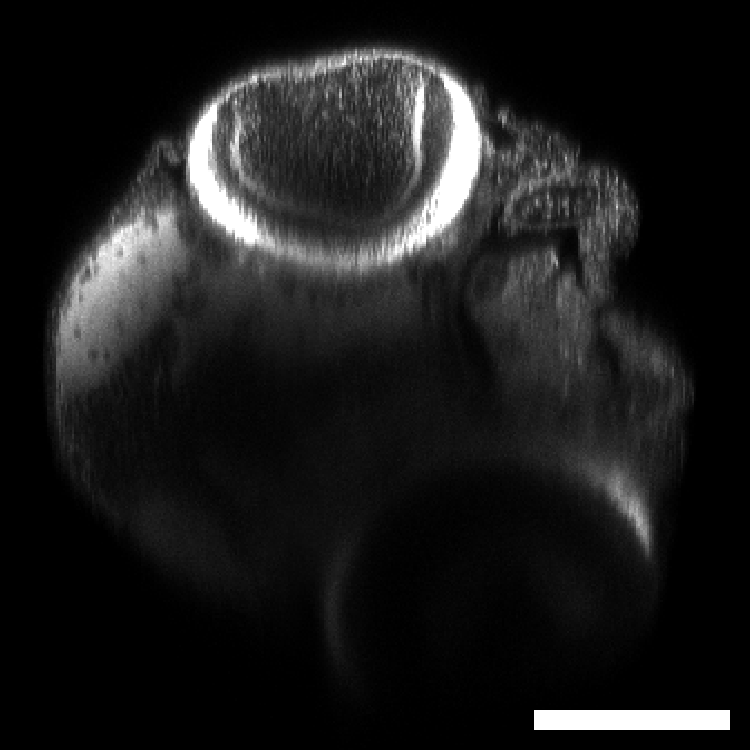
\includegraphics[width=\textwidth]{\Figures/sbddcc_original.png}
    \end{subfigure}
    \begin{subfigure}[b]{0.30\textwidth}
        \caption{
            \label{fig:sbddcc:niveaux}
        Carte\newline des profondeurs
            }
       \centering 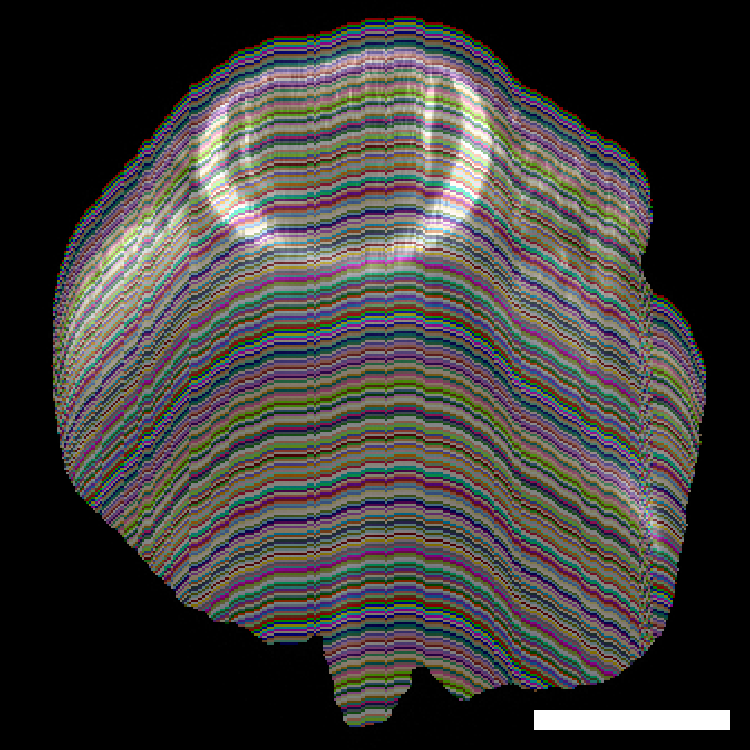
\includegraphics[width=\textwidth]{\Figures/sbddcc_niveaux.png}
    \end{subfigure}
    \begin{subfigure}[b]{0.30\textwidth}
        \caption{
            \label{fig:sbddcc:correction}
            \centering{
            Après SBDDCC
                }
            }
       \centering 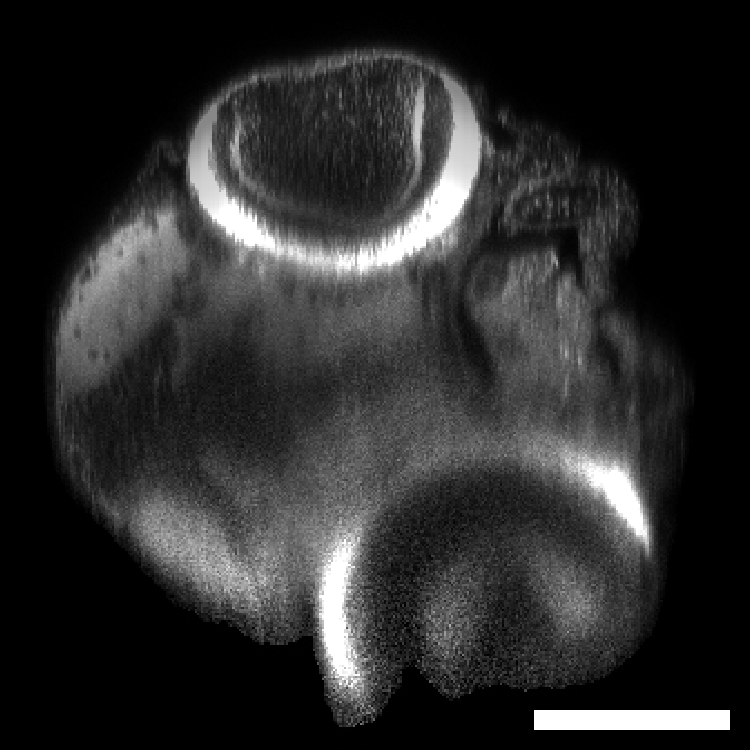
\includegraphics[width=\textwidth]{\Figures/sbddcc_corrige.png}
    \end{subfigure}
    \caption{
    Résultat de l'application du SBDDCC visualisé sur une coupe transversale d'alevins de \pz{}.
    \newline
    Cette algorithme commence par calculer le médian des valeurs de gris en fonction de la profondeur de tissus traversée.
    Cette fonction est ensuite utiliser pour normaliser les médians des couches profondes, ce qui permet de compenser l'atténuation lumineuse au sein de l'échantillon.
    \newline
    Barre d'échelle: 250~$\mu{}m$
    }
\end{center}
\end{figure}

\subsection{Un algorithme compensant la déperdition lumineuse en fonction de l'épaisseur des tissus traversés}

%
Considérons $I$ l'acquisition à traiter et $S_{\texnormal{larva}}$ la segmentation de la larve entière au sein de cette acquisition (Voir la \autoref{sec:algo:larva} pour une description de l'algorithme permettant la segmentation de la larve entière).

%
Soit $b$ le dernier plan de $I$ dans le sens de l'acquisition.
%
On calcule tout d'abord une somme cumulative de $S_{\texnormal{larva}}$ dans le sens de l'acquisition~\eqref{eq:sbddcc:cum_sum}.
%
On multiplie ensuite cette somme cumulative par $S_{\texnormal{larva}}$ pour obtenir une carte de la quantité de tissus à parcourir depuis le plan d'acquisition~\eqref{eq:sbddcc:carte}.
%
Soit $d$ une quantité de tissus à pénétrer quelconque, $d_b$ la plus grande quantité de tissus à pénétrer.

\begin{equation}
    \label{eq:sbddcc:cum_sum}
    \forall z \in [0;b], 
        C_1(z)=\sum_{n=1}^{z}S_{\textnormal{larva}}(n)
\end{equation}

\begin{equation}
    \label{eq:sbddcc:carte}
    C_2=C_1 * S_{\textnormal{larva}}
\end{equation}
%
On calcule la valeur de gris médiane des voxels de I se trouvant pour chaque couche.
%
Appelons $\mu{}(d)$ la valeur médiane de $I$ pour la couche $d$, $\mu_{max}$ la valeur maximale de $\mu{}(d)$ et $d_{max}$ l'indice de $\mu_{max}$ au sein de $\mu{}(d)$.
%
L'amélioration de contraste est réalisée en multipliant chaque valeur de gris au sein des couches $d$ plus grande que $d_{max}$ par $\mu_{max}$ divisé par $\mu_d$~\eqref{eq:sbddcc:correction}.

\begin{equation}
    \label{eq:sbddcc:correction}
    \forall d \in [d_{max};d_b],
        I_{c}(d)=I(d)*\frac{\mu_{\max}}{\mu(d)}
\end{equation}

\end{document}
